% main.tex

\section{Introduction}

\begin{chapquote}{Richard Feynman}
Everything is interesting if you go into it deeply enough.
\end{chapquote}

\noindent The title of this thesis is \emph{Exact Results in Supersymmetric Gauge Theories}. A reasonable question to ask is -- why would anyone care about that ? 
After all there is no evidence that supersymmetry is a true symmetry of nature and supersymmetric theories are mostly toy theories, we can not observe them in particle accelerators, as opposed to the Standard Model of particle physics. 
And indeed these are all valid points, however there are very good reasons for studying them. 

Consider $\N=4$ super Yang-Mills, from a pragmatic point of view it is the simplest non-trivial quantum field theory in four spacetime dimensions and since attempts at solving realistic QFTs such as the theory of strong interactions (QCD) have so far been futile, it seems like a good starting point -- some go as far as calling it the harmonic oscillator of QFTs. 

Another (and probably the main) reason why $\N=4$ has been receiving so much attention in the last decades is the long list of mysterious and intriguing properties it seems to posses, making it almost an intellectual pursuit of understanding it. 
The theory has been surprising the theoretical physics community from the very beginning: it is a rare instance of a conformal theory in dimensions higher than two, it has a dual description in terms of a string theory and more recently it was discovered to be integrable in the planar limit. 
All of these properties give reasonable hope for actually solving the theory exactly, something that has never been achieved before for any four dimensional interacting QFT.

In the remainder of the section we give a proper introduction to the subject from a historic point of view focusing on $\N=4$ SYM and its integrability aspect, for it is integrability that allows one to actually find exact results in the theory. We then give an overview of the thesis itself, emphasizing which parts of the text are reviews of known material and which parts constitute original work.

\subsection{Brief history of the subject}

Quantum field theory has been at the spot light of theoretical physics since the beginning of the century when it was found that electromagnetism is described by the theory of quantum electrodynamics (QED). Since then people have been trying to fit other forces of nature into the QFT framework. 
Ultimately it worked: the theory of strong interactions, quantum chromodynamics or QCD for short, together with the electroweak theory, spontaneously broken down to QED, collectively make up the \emph{Standard Model} of particle physics, which has been extensively tested in particle accelerators since then. 

However nature did not give away her secrets without a fight. 
For some time it was though that strong interactions were described by a theory of vibrating strings, as it seemed to incorporate the so-called Regge trajectories observed in experiments \cite{Veneziano:1968}. 
Even after discovering QCD, which is a Yang-Mills gauge theory, stringy aspects of it were still evident and largely mysterious. 
Most notably lattice gauge theory calculations at strong coupling suggested that surfaces of color-electric fluxes between quarks could be given the interpretation of stretched strings \cite{Wilson:1974}, thus an idea of a gauge-string duality was starting to emerge. 
It was strongly re-enforced by t'Hooft, who showed that the perturbative expansion of $U(N)$ gauge theories in the large $N$ limit could be rearranged into a genus expansion of surfaces triangulated by the double-line Feynman graphs, which strongly resembles string theory genus expansions \cite{THooft:1974}.

\vspace{20pt}
\newlength\yearposx
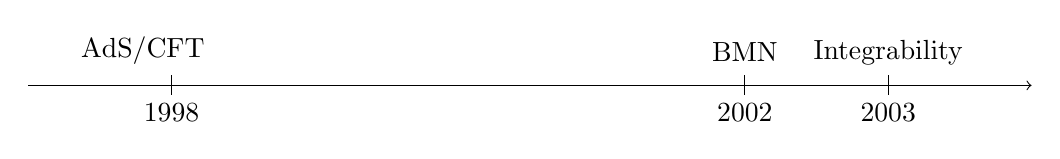
\begin{tikzpicture}[scale=1.82]

    \foreach \x in {1997,1998,2002,2003,2004}{
        \pgfmathsetlength\yearposx{(\x-1996)*1cm};
        \coordinate (y\x)   at (\yearposx,0);
        \coordinate (y\x t) at (\yearposx,+2pt);
        \coordinate (y\x b) at (\yearposx,-2pt);
    }
	
    \draw [->] (y1997) -- (y2004);
    \foreach \x in {1998,2002,2003} \draw (y\x t) -- (y\x b);

	\node at (y1998) [below=3pt] {1998}; 
		\node at (1.8cm, 0) [above=4pt] {AdS/CFT}; 
	\node at (y2002) [below=3pt] {2002}; \node at (y2002) [above=5pt] {BMN}; 
	\node at (y2003) [below=3pt] {2003}; \node at (y2003) [above=4pt] {Integrability}; 
\end{tikzpicture}
\vspace{20pt}

However it was the work of Maldacena in the end of 1997 that sparked a true revolution in the field \cite{Maldacena:1997re}. 
He formulated the first concrete conjecture, now universally referred to as \emph{AdS/CFT}, for a duality between a gauge theory, the maximally supersymmetric $\N=4$ super Yang-Mills, and type IIB string theory on $\adsfive$. 
Polyakov had already shown that non-critical string theory in four-dimensions describing gauge fields should be complemented with an extra Liouville-like direction thus enriching the space to a curved five dimensional manifold \cite{Polyakov:1997tj}. Furthermore the gauge theory had to be defined on the boundary of this manifold.
Maldacena's conjecture was consistent with this view, as the gauge theory was defined on the boundary of $AdS_5$, whereas the $S^5$ was associated with the internal symmetries of the gauge fields.
The idea of a higher dimensional theory being fully described by a theory living on the boundary was also considered before in the context of black hole physics \cite{'tHooft:1993gx, Susskind:1994vu} and goes by the name of holography, thus AdS/CFT is also referred to as a holographic duality.

The duality can be motivated by considering a stack of $N$ parallel D3 branes in type IIB string theory. 
Open strings moving on the branes can be described by $\N=4$ SYM with the gauge group $SU(N)$. 
Roughly the idea is that there are six extra dimensions transverse to the stack of branes, thus a string stretching between two of them can be viewed as a set of six scalar fields ${(\Phi^i)^a}_b$ defined in four dimensional spacetime carrying two extra indices denoting the branes it is attached to. 
These are precisely the indices of the adjoint representation of $SU(N)$.
A similar argument can be put forward for other fields thus recovering the field content of $\N=4$ SYM.
Far away from the branes we have closed strings propagating in empty space. 
In the low energy limit these systems decouple and far away from the branes we are left with ten dimensional supergravity.

Another way of looking at this system is considering the branes as a defect in spacetime, which from the point of view of supergravity is a source of curvature. 
The supergravity solution carrying D3 brane charge can be written down explicitly \cite{Horowitz:1991cd}.
Far away from the branes it is obviously once again the usual flat space ten dimensional supergravity.
However the near horizon geometry of the brane system becomes $\adsfive$.
Since both points of view end up with supergravity far away from the branes, one is tempted to identify the theories close to the branes, $\N=4$ SYM and type IIB string theory on $\adsfive$. 
This is exactly what Maldacena did in his seminal paper \cite{Maldacena:1997re}. 

By studying the supergravity solution one can identify the parameters of the theories, namely $\N=4$ SYM is parametrized by the coupling constant $g_{YM}$ and the number of colors $N$, whereas string theory has the string coupling constant $g_s$ and the string length squared $\alpha'$. 
These are identified in the following way
\beq
	 4\pi g_s = g_{YM}^2 \equiv \frac{\lambda}{N}, \;\;\;\;\;\;\; \frac{R^4}{\alpha'^2} = \lambda,
\eeq
where $\lambda$ is the t'Hooft coupling and $R$ is the radius of both $AdS_5$ and $S_5$, which is fixed as only the ratio $R^2/\alpha'$ is measurable.
A few things are to be noted here. First of all, the identification directly implements t'Hooft's idea of large $N$ expansion of gauge theory, since $g_s \sim 1/N$. 
In fact in the large $N$ limit only planar Feynman graphs survive and everything simplifies dramatically, a fact that we will take advantage of a lot in this thesis.
In this limit the effective coupling constant of the gauge theory is $\lambda$. 

The supergravity approximation is valid when $\alpha' \ll R^2$, which corresponds to strongly coupled gauge theory, thus the conjecture is of the weak-strong type. 
This fact is a blessing in disguise, since initially it seems very restrictive as one can not easily compare results of the theories. 
However it provides a possibility to access strongly coupled regimes of both theories, which was beyond reach before. 
Prescriptions for matching up observables on both sides of the correspondence were given in \cite{Gubser:1998bc, Witten:1998qj}. 
However because of the weak-strong nature of the duality initial tests were performed only for BPS states, which are protected from quantum corrections.
The first direct match was observed in \cite{Witten:1998qj} where it was shown that the spectrum of half-BPS single trace operators matches the Kaluza-Klein modes of type IIB supergravity.
Another indirect confirmation of the conjecture was the formulation of type IIB string theory as a super-coset sigma model on the target space $PSU(2,2|4) / SO(2,4) \otimes SO(6)$, which has the same global symmetries as $\N=4$ SYM \cite{Metsaev:1998it}.

The situation changed dramatically in 2002 when Berenstein, Maldacena and Nastase devised a way to go beyond BPS checks \cite{Berenstein:2002jq}. 
The idea was to take an operator in gauge theory with large R-charge $J$ and add some some impurities, effectively making it ``near-BPS''.
The canonical example of such an operator is $\tr(Z^J X^S)$, where $Z$ and $X$ are two complex scalar fields of $\N=4$ SYM, with $X$ being the impurities ($S \ll J$).
Since anomalous dimensions are suppressed like $\lambda/J^2$, perturbative gauge theory calculations are valid even at large $\lambda$, as long as $\lambda' \equiv \lambda / J^2 \ll 1$ and $N$ is large.
It is thus possible to compare gauge theory calculations with string theory results.
From the string theory point of view this limit corresponds to excitations of point-like strings with angular momentum $J$ moving at the speed of light around the great circle of $S^5$. 
The background seen by this string is the so-called pp-wave geometry and string theory in this background is tractable.

The discovery of the BMN limit was arguably the first time it was explicitly demonstrated how the world sheet theory of a string can be reconstructed by a physical picture of scalar fields dubbed as ``impurities'' propagating in a closed single trace operator of ``background'' scalar fields of the gauge theory. 
Shortly after this discovery Minahan and Zarembo revolutionized the subject once again by discovering Integrability at the end of 2002 \cite{Minahan:2002ve}.
They showed that in the large $N$ limit single-trace operators of scalar fields can be identified with spin chains and their anomalous dimensions at one-loop in weak coupling are given by the energies of the corresponding spin chain states.
These spin-chain systems are known to be integrable, which in practice allows one to solve the problem exactly using techniques such as the Bethe ansatz \cite{Bethe:1931}. 
This discovery sparked a very rapid development of integrability methods in AdS/CFT during the coming years.

\vspace{20pt}
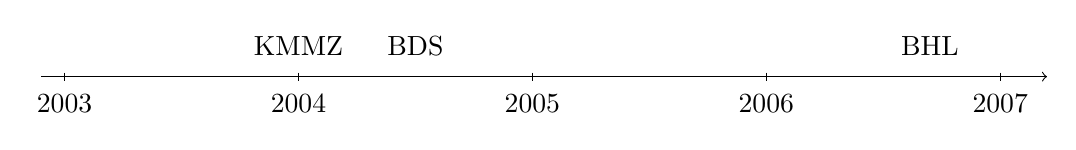
\begin{tikzpicture}[scale=2.97]
    
	\coordinate (start) at (0,0);
	\coordinate (end) at (4.3cm,0);
	
    \foreach \x in {2003,2004,2005,2006,2007}{
        \pgfmathsetlength\yearposx{((\x-2003)*1cm + 0.1cm)};
        \coordinate (y\x)   at (\yearposx,0);
        \coordinate (y\x t) at (\yearposx,+0.5pt);
        \coordinate (y\x b) at (\yearposx,-0.5pt);
    }
	
    \draw [->] (start) -- (end);
    \foreach \x in {2003,2004,2005,2006,2007} \draw (y\x t) -- (y\x b);

	\node at (y2003) [below=3pt] {2003}; 
		\node at (0.5cm, 0) [above=4pt] {}; 
	\node at (y2004) [below=3pt] {2004}; 
		 \node at (y2004) [above=4pt] {KMMZ}; 
	\node at (y2005) [below=3pt] {2005}; 
		 \node at (1.6cm, 0) [above=4pt] {BDS}; 
	\node at (y2006) [below=3pt] {2006}; 
		 \node at (3.8cm, 0) [above=4pt] {BHL}; 
	\node at (y2007) [below=3pt] {2007}; 
\end{tikzpicture}
\vspace{20pt}

Solving a quantum field theory in principle means finding all $n$-point correlation functions of all physical observables. 
Since $\N=4$ SYM is conformal it is enough to find all 2-point and 3-point correlators, as all higher point correlation functions can be decomposed in terms of these basic constituents.
Due to conformal symmetry the two-point functions only depend on the scaling dimensions of operators, whereas for three point functions one also needs the so called structure constants $C_{ijk}$ in addtion to the scaling dimensions.
Integrability methods from the very beginning mainly focused on solving the spectral problem in the large $N$ limit, that is finding the spectrum of operators with definite anomalous dimensions and their exact numeric values.
The initial discovery of \cite{Minahan:2002ve} was that the spectral problem was analogous to diagonalizing a spin chain Hamiltonian, which was identified with the dilatation operator of the superconformal symmetry of the theory.
The eigenstates correspond to operators in the gauge theory and the eigenvalues are their anomalous dimensions.

Soon after the initial discovery of integrability a spin chain formulation at one-loop was found for the full $PSU(2,2|4)$ theory, not only the scalar sector \cite{Beisert:2003jj}. 
The result was also extended to two and three loops \cite{Beisert:2003tq}. 
Integrability was also discovered at strong coupling as it was shown that the Metsaev-Tseytlin sigma model is classically integrable \cite{Bena:2003wd}. 
With integrability methods now being available at both weak and strong coupling it was possible to compare results in the BMN limit.
As expected, comparisons in the first two orders of the BMN coupling constant $\lambda'$ showed promising agreement \cite{Frolov:2003qc, Frolov:2003xy, Arutyunov:2003uj}, however an order of limits problem emerged at three loops \cite{Beisert:2003tq}. 

All of these results seemed to suggest that integrability may be an all loop phenomenon, only the surface of it being scratched so far. 
This notion was strongly reinforced when classical string integrability was reformulated in the elegant language of algebraic curves by Kazakov, Marshakov, Minahan and Zarembo (KMMZ), which made the connection with weak coupling more manifest \cite{Kazakov:2004qf}. 
The algebraic curve was interpreted as the continuum limit of Bethe equations, which made it possible to speculate about all loop equations.
The first such attempt was made by Beisert, Dippel and Staudacher (BDS), who conjectured a set of Bethe equations and a dispersion relation which together successfully showcased some all-loop features \cite{Beisert:2004hm}.
This result was later extended to all sectors of the theory \cite{Beisert:2005fw}.
The BDS result was quickly shown to be incomplete as it was lacking a so-called dressing phase \cite{Arutyunov:2004vx}, a scalar function not constrained by symmetry of the problem.
It was found to leading order at strong coupling in \cite{Arutyunov:2004vx} and later to one-loop in \cite{Hernandez:2006tk}.
A crossing equation satisfied by the dressing phase was soon found \cite{Janik:2006dc} and eventually solved by Beisert, Hernandez and Lopez (BHL) \cite{Beisert:2006ib}.  
Collectively these results are often referred to as the asymptotic Bethe ansatz (ABA), reminding that they are valid only for asymptotically long spin chains. 
When the states are short so-called wrapping effects become relevant. 
At weak coupling they manifest as long-range spin chain interactions wrapping around the chain, whereas at strong coupling they are due to virtual particles self-interacting across the circumference of the worldsheet \cite{Sieg:2005kd, Ambjorn:2005wa}.

\vspace{20pt}
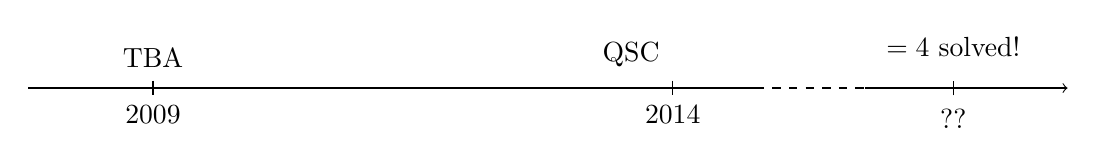
\begin{tikzpicture}[scale=1.32]

	\coordinate (start) at (0,0);
	\coordinate (end) at (6.5cm,0);
	
    \foreach \x in {2009,2010,2012,2014}{
        \pgfmathsetlength\yearposx{(\x-2008)*1cm + 0.2cm};
        \coordinate (y\x)   at (\yearposx,0);
        \coordinate (y\x t) at (\yearposx,+2pt);
        \coordinate (y\x b) at (\yearposx,-2pt);
    }
    
    \draw [-] (0,0) -- (7cm,0);
    %\draw [decorate, decoration={snake, segment length=5mm, amplitude=1mm}, dashed] (7cm,0) -- (8.05cm,0);
	\draw [-, dashed] (7cm,0) -- (8.05cm,0);
	\draw [->] (8.05cm,0) -- (10cm,0);
	
	\foreach \x in {2009,2014} \draw (y\x t) -- (y\x b);
	
    \node at (y2009) [below=3pt] {2009}; \node at (y2009) [above=4pt] {TBA}; 
	\node at (y2014) [below=3pt] {2014}; 
		\node at (5.8cm, 0) [above=4pt] {QSC}; 
		
	\draw (8.9cm,-2pt) -- (8.9cm,+2pt);
	\node at (8.9cm,0) [below=4pt] {??}; \node at (8.9cm,0) [above=8pt] {$\N=4$ solved!}; 
	
\end{tikzpicture}
\vspace{20pt}

Once the asymptotic solution was found attention shifted to finite size corrections, which once resolved would in principle complete the solution to the spectral problem for single trace operators. 
Scattering corrections in finite volume for arbitrary QFTs were first addressed by L\"{u}scher \cite{Luscher:1986}, who derived a set of universal formulas. 
This approach, while very general and not directly related to integrability, was employed to calculate four \cite{Bajnok:2008bm} and five loop anomalous dimension coefficients \cite{Bajnok:2009vm} of the simplest non-BPS operator with length two, the Konishi operator.
The results agreed with available diagrammatic four-loop calculations \cite{Fiamberti:2007rj} and gave a new prediction for five loops.

An alternative approach more in line with integrability is the Thermodynamic Bete Ansatz (TBA).
Its origins can be traced back to Yang and Yang \cite{Yang}, however it was the work of Alexey Zamolodchikov \cite{Zamolodchikov1, Zamolodchikov2} that brought it to the mainstream. 
The idea is to consider the partition function of a two dimensional integrable CFT and it's ``mirror'' image found after exchanging length and time with a modular transformation.
At large imaginary times the partition function will be dominated by the ground state energy, whereas in the mirror theory large time means asymptotic length, which is under control using the asymptotic Bethe ansatz techniques.
Thus one can evaluate the partition function using the saddle point method and after rotating back to the original theory compute the exact ground state energy. 
Excited states can then be reached using analytic continuation. 
This approach was already proposed as an option for the AdS/CFT system in \cite{Ambjorn:2005wa} and was first discussed in depth in \cite{Arutyunov:2007tc}.
The TBA approach crystallized in 2009 with multiple groups publishing results almost simultaneously \cite{Gromov:2009tv, Bombardelli:2009ns, Gromov:2009bc, Arutyunov:2009ur}.
The Konishi anomalous dimension was initially checked at four \cite{Gromov:2009bc} and five \cite{Arutyunov:2010gb, Balog:2010xa} loops by linearising the TBA equations, showing precise agreement with results obtained using the L\"{u}scher method.
Ultimately the Konishi anomalous dimension was calculated numerically for a wide range of values of the t'Hooft coupling constant \cite{Gromov:2009zb}.

And so the spectral problem seemed to be solved, at least in the case of Konishi an exact and complete result was finally found, even if only numerically.
However it was increasingly becoming clear that the solution was not in its final and most elegant form.
Indeed the TBA equations are an infinite set of coupled integral equations, obviously one has to employ various numerical tricks to actually solve them and this mostly works in a case-by-case basis. 
Cases such as the $\mathfrak{sl}(2)$ sector of the theory, containing the Konishi operator \cite{Gromov:2009bc} and cusped Wilson lines \cite{Correa:2012hh, Gromov:2012eu} have been worked out explicitly, however it still remains a hard problem in general.
From the very beginning alternative formulations of the solution were being proposed. 
An infinite set of non-linear functional equations, the so called Y-system was proposed already in \cite{Gromov:2009bc}, later completed with analytical constraints coming from the TBA equations \cite{Cavaglia:2010nm}.
Connections of the Y-system with the Hirota bilinear relation were later explored in \cite{Gromov:2011cx} and the Y-system was reduced to a finite set of non-linear integral equations (FiNLIE).
The long sought beauty of the solution to the spectral problem was arguably uncovered with the formulation of the quantum spectral curve (QSC) approach \cite{Gromov:2013pga,Gromov:2014caa}, also referred to as the $\pmu$-system.
The whole TBA construction was ultimately reduced to a Riemann-Hilbert problem for eight $Q$ functions, which can be though of as the quantum analogues of quasimomenta found in the algebraic curve construction.
The QSC quickly showed its potential as previously known results were rederived almost without any effort and new results were being rapidly discovered \cite{Gromov:2013qga, Gromov:2014bva}.

Thus one can safely say that the spectral problem in $\N=4$ SYM is by now very well understood with numerical results readily available and deeper understanding of the structure being within reach.
Integrability methods have also been useful in other areas such as three point functions \cite{Escobedo:2010xs, Gromov:2012vu} and scattering amplitudes \cite{Drummond:2010km, Alday:2010kn}, however the situation there is still not as complete.
Having witnessed the successful resolution of the spectral problem it appears that $\N=4$ SYM is within reach of being solved completely.
If this programme were to be successfully carried out it would be the first example of a four dimensional interacting quantum field theory being solved exactly.
Undoubtedly this would provide a huge boost to our understanding of QFTs in general and hopefully bring us closed to solving QCD.

It turns out that $\N=4$ SYM is not the only example of an integrable supersymmetric gauge theory having a dual string description.
Probably the most famous example involves the so called ABJM theory, proposed by Aharony, Bergman, Jafferis and Maldacena \cite{Aharony:2008ug}, following \cite{Schwarz:2004yj, Bagger:2006sk, Gaiotto:2007qi}.
It is a three-dimensional superconformal Chern-Simons gauge theory with $\N=6$ supersymmetry.
This theory was conjectured to be the effective theory for a stack of M2 branes at a $Z_k$ orbifold
point. 
In the large $N$ limit its gravitational dual turns out to be M-theory on $AdS_4 \times S^7 / Z_k$. 
For large $k$ and $N$ with $\lambda = N/k$ fixed, the dual theory becomes type IIA superstring theory in $AdS_4 \times CP^3$.
This duality is also integrable \cite{Minahan:2008hf} and all of the developments outlined above have been reworked for it almost in parallel. 

\newpage
\subsection{Thesis overview}

The thesis consists of four core chapters, the first three of which cover $\N=4$ super Yang-Mills.
We start by introducing the theory in chapter \ref{sec:cft} where we give its field content, Lagrangian and talk briefly about symmetries and their representations.
We introduce the dual string theory in section \ref{sec:n4_strong} and talk briefly about its formulation as a super-coset sigma model.

Chapter \ref{sec:integrability} covers integrable structures found in $\N=4$ super Yang-Mills at strong and weak coupling, namely we discuss the spin chain picture at weak coupling in section \ref{sec:integrability_weak} and the algebraic curve picture found at strong coupling in section \ref{sec:integrability_strong}.
A lot of focus in this chapter is put on the folded string solution described in section \ref{sec:folded_string}. 
It is the strong coupling dual to operators in the $\alg{sl}{2}$ sector of $\N=4$ super Yang-Mills, which are described in section \ref{sec:sl2_sector}. 
A key result of the chapter is the calculation of the Konishi anomalous dimension up to two loops at strong coupling achieved by boosting the one-loop result with the help of the exact slope function found in section \ref{sec:slope_function_aba}.

In chapter \ref{sec:exact_results} we move away from the perturbative regime and introduce exact solution methods for the spectral problem of $\N=4$ super Yang-Mills -- the thermodynamic Bethe ansatz and Y/T-systems in section \ref{sec:tba_y_system} and the novel quantum spectral curve construction in section \ref{sec:pmu_system}.
We then discuss exact solutions found using the quantum spectral curve, the first one being the anomalous dimension of a cusped Wilson line in section \ref{sec:wilson_line}, the classical limit is also discussed in \ref{sec:wilson_classical}.
The slope function is rederived in section \ref{sec:slope_pmu} and the calculation is extended one order further to find the curvature function in \ref{sec:curvature}.
The chapter concludes by revisiting the Konishi anomalous dimension in section \ref{sec:konishi_three_loops} and using the curvature function to boost the previously obtained two-loop strong coupling result to three loops.
 
Chapter \ref{sec:abjm} switches over from $\N=4$ super Yang-Mills to the ABJM theory and roughly follows the same path, however as most of the methods are very similar in spirit we move on much quicker.
We introduce the theory in section \ref{sec:abjm_intro} and discuss integrability in section \ref{sec:abjm_integrability}. 
Section \ref{sec:abjm_folded} describes the analogue of the folded string solution in ABJM, in particular the semi-classical quantization procedure of the solution.
We finish with a short overview of exact results in section \ref{sec:abjm_exact}.

We end with conclusions and appendices containing some of the more technical details left out from the main text for brevity.
The interdependencies between the chapters and sections of the text are shown in figure \ref{fig:chapters}.

%\vspace{30pt}
\newpage
\subsection{Original work}

The thesis contains original work by the author from five papers published in collaboration with fellow colleagues while working towards the PhD degree. 
Section \ref{sec:short_strings} is based on \cite{Gromov:2011bz}, where the two-loop strong coupling Konishi anomalous dimension was first calculated.
The calculation relied on semi-classical quantization of the folded string solution in $\N=4$ super Yang-Mills, the exact analogous calculation was then performed by the author in \cite{Beccaria:2012vb,Beccaria:2012qd} for the ABJM theory, which is the basis for section \ref{sec:abjm_folded}.
Section \ref{sec:wilson_classical} describing the classical limit of the cusped Wilson line is based on \cite{Sizov:2013joa}.
The remainder of chapter \ref{sec:exact_results} concerning the slope and curvature functions and their use to find the three-loop Konishi anomalous dimension at strong coupling are based on the work done in \cite{Gromov:2014bva}. 

Naturally in order to achieve a uniform flow throughout the text we introduced some filler sections outlining the basics of techniques we utilize later. 
These sections are kept short and are thoroughly filled with references to original work and/or reviews of the subject matter.
We hope the reader is not offended or annoyed by the inhomogeneous level of detail in various sections of the text and enjoys the thesis!

\vspace{60pt} 
 
\begin{figure}[h]
\centering
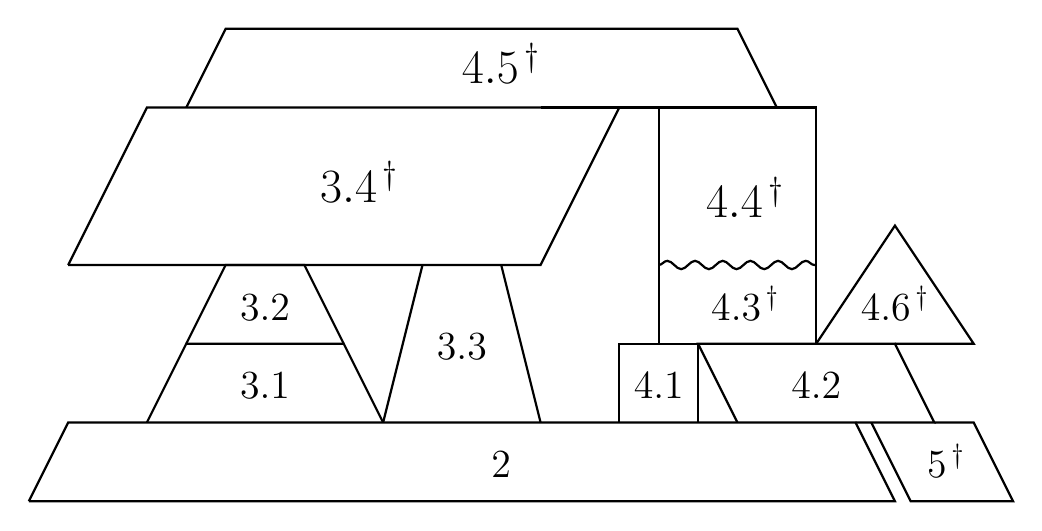
\begin{tikzpicture}[scale=1]
	
	%\draw[help lines] (0,0) grid (13,6);
	
	\draw[thick] (0.5, 0) -- (11.5, 0) -- (11, 1) -- (1, 1) -- (0.5, 0); % 2
	\node at (6.5, 0) [above=5] {\Large 2};  
	
	\draw[thick] (11.2, 1) -- (11.7, 0) -- (13, 0) -- (12.5, 1) -- (12, 1); % 5
	\node at (12.15, 0) [above=5] {\Large $5^{\,\dagger}$}; 
	
	\draw[thick] (2, 1) -- (2.5, 2) -- (4.5, 2) -- (5, 1); % 3.1
	\node at (3.5, 1) [above=5] {\Large 3.1}; 
	
	\draw[thick] (2.5, 2) -- (3, 3) -- (4, 3) -- (4.5, 2); % 3.2
	\node at (3.5, 2) [above=5] {\Large 3.2}; 
	
	\draw[thick] (5, 1) -- (5.5, 3); % 3.3
	\draw[thick] (6.5, 3) -- (7, 1); % 3.3
	\node at (6, 1.5) [above=5] {\Large 3.3}; 
	
	\draw[thick] (1, 3) -- (7, 3) -- (8, 5) -- (2, 5) -- (1, 3); % 3.4
	\node at (4.7, 3.5) [above=5] {\LARGE $3.4^{\,\dagger}$}; 
	
	\draw[thick] (8, 1) -- (8, 2) -- (9, 2) -- (9, 1); % 4.1
	\node at (8.5, 1) [above=5] {\Large 4.1}; 
	
	\draw[thick] (9.5, 1) -- (9, 2) -- (11.5, 2) -- (12, 1) -- (11, 1); % 4.2
	\node at (10.5, 1) [above=5] {\Large 4.2}; 
	
	\draw[thick] (8.5, 2) -- (8.5, 3.5); % 4.3
	\draw [decorate, decoration={snake, segment length=10, amplitude=1.5}, thick] (8.5, 3) -- (10.5, 3);
	\draw[thick] (10.5, 3.5) -- (10.5, 2); % 4.3
	\node at (9.6, 2) [above=5] {\Large $4.3^{\,\dagger}$}; 
	
	\draw[thick] (8.5, 3.5) -- (8.5, 5) -- (10.5, 5) -- (10.5, 3.5); % 4.4
	\node at (9.6, 3.3) [above=5] {\LARGE $4.4^{\,\dagger}$}; 
	
	
	\draw[thick] (10.5, 2) -- (11.5, 3.5) -- (12.5, 2) -- (11.5, 2); % 4.6
	\node at (11.5, 2) [above=5] {\Large $4.6^{\,\dagger}$}; 
	
	\draw[thick] (2.5, 5) -- (3, 6) -- (9.5, 6) -- (10, 5);
	\draw[thick] (7, 5) -- (8.5, 5); % 4.5
	\node at (6.5, 5) [above=5] {\LARGE $4.5^{\,\dagger}$}; 

\end{tikzpicture}
\caption{The interdependencies of the chapters and sections in the thesis. Sections containing mostly original work are marked with daggers.}
\label{fig:chapters}
\end{figure}
 
 
 
 
 
 
